Para a implementação do código que controla o robô, foram
utilizados dois métodos: o (1) \textit{Vector Field Histogram} (VFH)
\cite{c1}; e a técnica de (2) \textit{Bubble Band} \cite{c3}.
\\

\subsection{VFH}
\label{sec:vfh}

O VFH é um método desenvolvido para robôs-móveis evitarem obstáculos em tempo real, permitindo a
detecção de obstáculos desconhecidos ao mesmo tempo em que o robô se desvia destes em direção
ao objetivo. Em uma primeira etapa, o método utiliza uma grade de histograma cartesiano bidimensional $C$ para a representação dos obstáculos, que é frequentemente atualizada a cada taxa de dados amostrados pelos sensores do robô enquanto ele se move. Cada célula $(i,j)$ na grade de histograma contém um valor $c_{i,j}$, que representa a probabilidade de existir um obstáculo naquele local. A cada leitura de amostras, apenas uma célula a uma distância $d$ do sensor terá seu valor incrementado, resultando em um histograma de distribuição de probabilidade, no qual valores de alta certeza estarão em células próximas à atual posição de um obstáculo. A Figura \ref{fig:histog_dist_prob} mostra o quanto esta tática faz com que a mesma célula e as suas vizinhas sejam repetidamente incrementadas.

\begin{figure}[H]
    \centering
    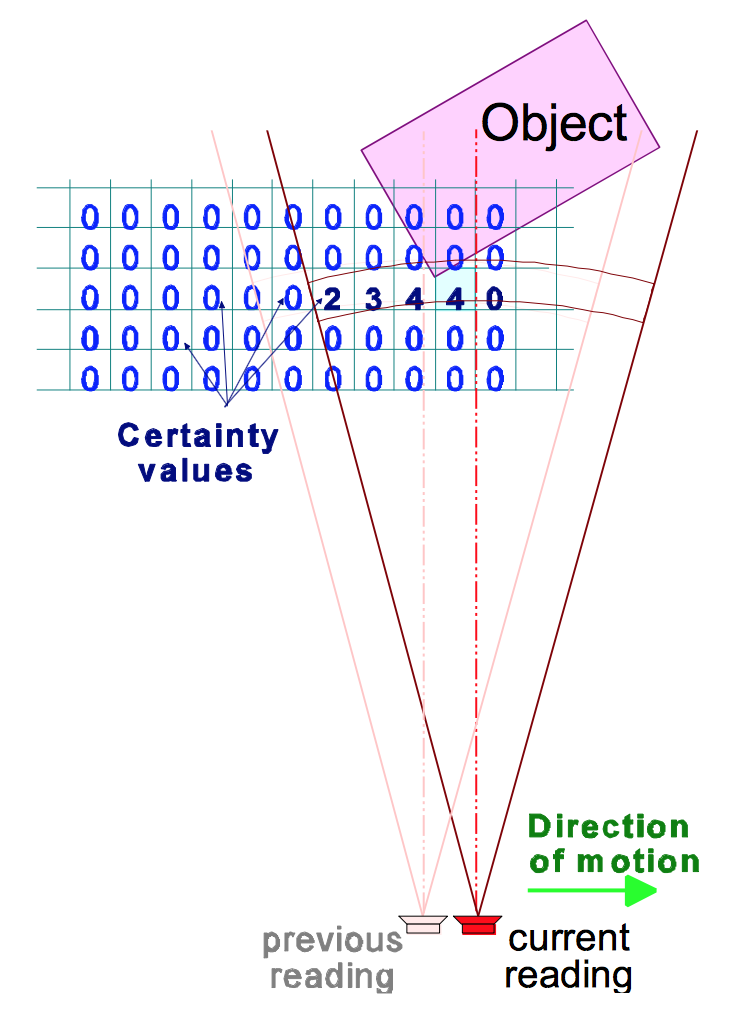
\includegraphics[width=0.4\textwidth]{img/histog_dist_prob}
    \caption{Histograma de distribuição de probabilidade. Fonte: \cite{c1}}
    \label{fig:histog_dist_prob}
\end{figure}

Em seguida, em uma etapa intermediária, a grade de histograma $C$ é reduzida em um histograma polar unidimensional $H$, que é construído de acordo com a localização momentânea do robô. $H$ consiste em $n$ setores de largura $\alpha$, cujo conteúdo é um valor que representa a densidade do obstáculo polar naquela direção. O mapeamento de $C$ em $H$ (Figura \ref{fig:map_grid_polar}) é realizado da seguinte forma: existe em $C$ uma janela de $w_{s} \times w_{s}$ células que se move junto do robô, chamada de região ativa $C^{*}$. As células ativas serão tratadas como um vetor de obstáculo, cuja direção $\beta$ será a medida da direção da célula até o centro do veículo. Desse modo, a direção $\beta$ é determinada por

\begin{figure}[H]
    \centering
    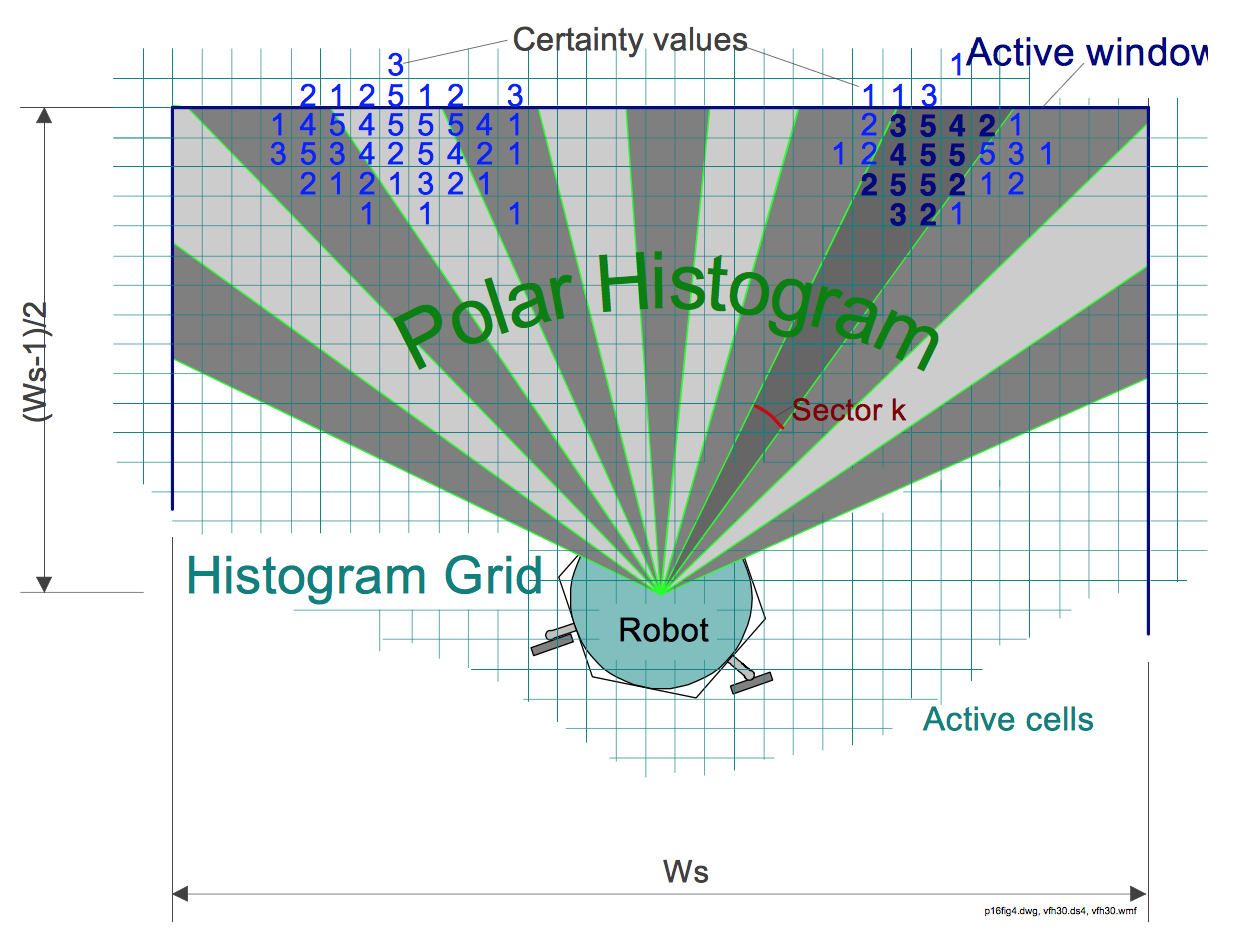
\includegraphics[width=0.8\textwidth]{img/map_grid_polar}
    \caption{Mapeamento das células ativas para o histograma polar $H$. Fonte: \cite{c1}}
    \label{fig:map_grid_polar}
\end{figure}

$$\beta = \tan^{-1}\frac{y_{i}-y_{0}}{x_{i}-x_{0}}$$

onde $x_{0}$ e $y_{0}$ são as coordenadas do centro do robô e $x_{i}$ e $y_{i}$ são as coordenadas da célula ativa $(i,j)$.
\\

A magnitute do vetor de obstáculo será dada por

$$m_{i,j} = (c^{*}_{i,j})^{2} (a - bd_{i,j})$$

onde $c^{*}_{i,j}$ é o valor de certeza da célula ativa $(i,j)$, $d_{i,j}$ é a distância entre a célula ativa $(i,j)$ e o centro do robô e $a$,$b$ são constantes positivas.
\\

A correspondência entre $c^{*}_{i,j}$ e o setor $k$ de $H$ é determinada através de

$$k = INT(\frac{\beta_{i,j}}{\alpha})$$

Para cada setor $k$, a densidade do obstáculo polar $h_{k}$ é calculada por

$$h_{k} = \sum_{i,j} m_{i,j}$$
\\

O resultado desse mapeamento pode gerar erros devido à natureza discreta da grade de histograma, por isso uma função de suavização é aplicada em $H$, obtendo a densidade de obstáculo polar suavizada $h'_{k}$ (POD).
\\

Nas Figuras \ref{fig:config_obs_grid_histog} e \ref{fig:polar_histog} é mostrado um exemplo de como essas duas etapas, a inicial e intermediária, são construídas.

\begin{figure}[H]
\centering
\begin{minipage}{.5\textwidth}
  \centering
  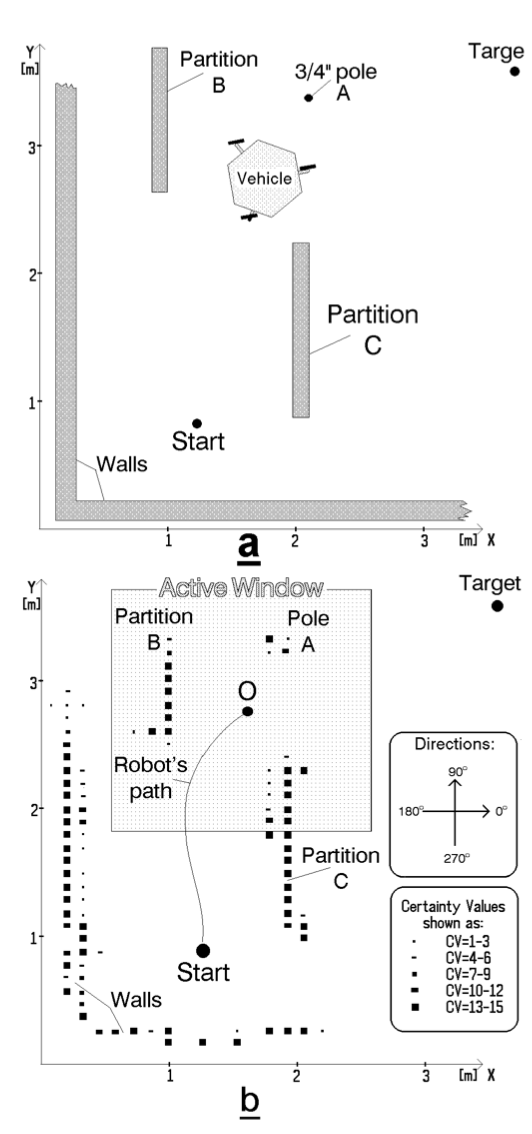
\includegraphics[width=.8\linewidth]{img/config_obs_grid_histog}
  \captionof{figure}{\textbf{a.} Exemplo de uma configuração de obstáculos. \textbf{b.} A representação da grade de histograma correspondente a o que está em \textit{a}. Fonte: \cite{c1}}
  \label{fig:config_obs_grid_histog}
\end{minipage}%
\begin{minipage}{.5\textwidth}
  \centering
  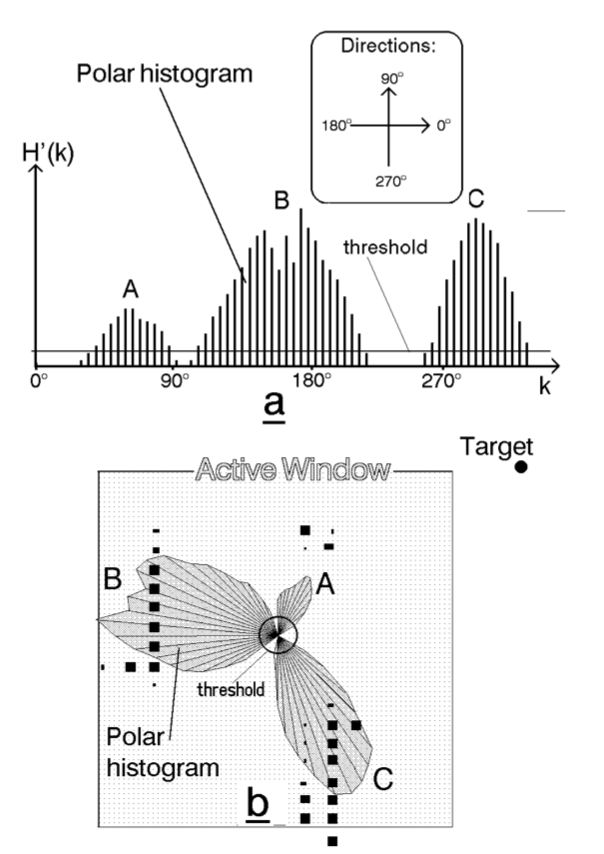
\includegraphics[width=.8\linewidth]{img/polar_histog}
  \captionof{figure}{\textbf{a.} A representação da densidade do obstáculo polar no histograma polar $H$ relativa à posição do robô em $O$. \textbf{b.} O histograma polar mostrado em \textit{a} na forma polar sobreposto pela grade de histograma mostrada na Figura \ref{fig:config_obs_grid_histog}b Fonte: \cite{c1}}
  \label{fig:polar_histog}
\end{minipage}
\end{figure}

%\begin{figure}[H]
%    \centering
%    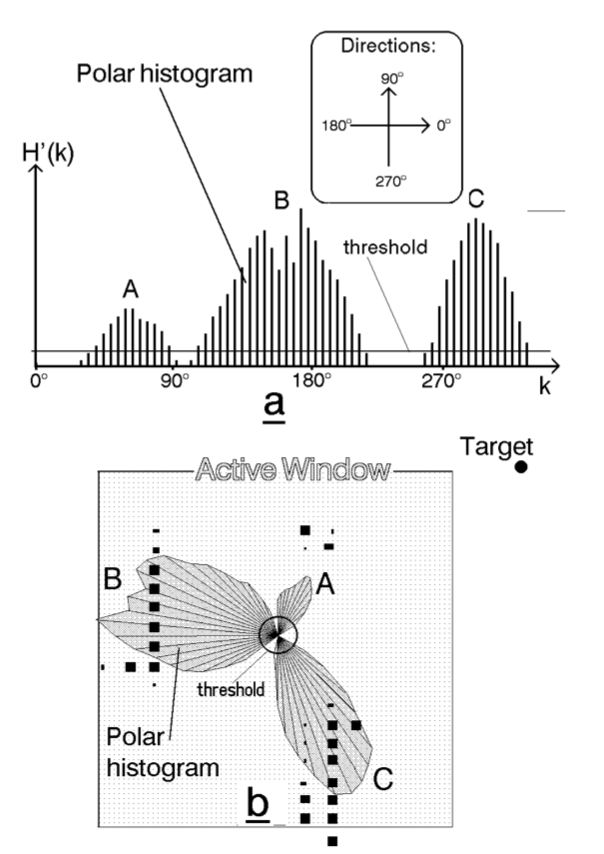
\includegraphics[width=0.55\textwidth]{img/polar_histog}
%    \caption{Histograma polar de magnitudes, com um valor empírico de limiar(threshold) de definição de um vale. Fonte: \cite{c1}}
%    \label{fig:polar_histog}
%\end{figure}

Na última etapa do método VFH, é computada a saída do algoritmo, que é a direção $\theta$ necessária para o robô girar se desviando do obstáculo.
\\

Um histograma polar possui "picos", setores com altos PODs,  e "vales", setores com baixos PODs. Qualquer \textit{vale} pertencente a um certo limiar é chamado de \textit{vale candidato}. Geralmente, há dois ou mais \textit{vales candidatos} e o algoritmo escolhe aquele que mais corresponde com a direção do objetivo $k_{targ}$.	 Uma vez que um \textit{vale} é escolhido, é necessário encontrar um setor apropriado do \textit{vale}.

O algoritmo mede a quantidade de setores no \textit{vale} para determinar se ele é um \textit{vale} \textit{largo} ou \textit{estreito}. Um \textit{vale largo} ocorre quando seu número de setores consecutivos dentro do limiar ultrapassou o valor $s_{max}$. O setor mais próximo de $k_{targ}$ é denotado por $k_{n}$ e $k_{f}$ é definido por $k_{f} = k_{n}+s_{max}$, ficando mais longe da borda. A direção de giro $\theta$ desejada é calculada por $\theta = \frac{(k_{n} + k_{f})}{2}$. Na Figura \ref{fig:cand_direc} é mostrado um exemplo de quais direções podem ser escolhidas para que um robô contorne os obstáculos. 

\begin{figure}[H]
    \centering
    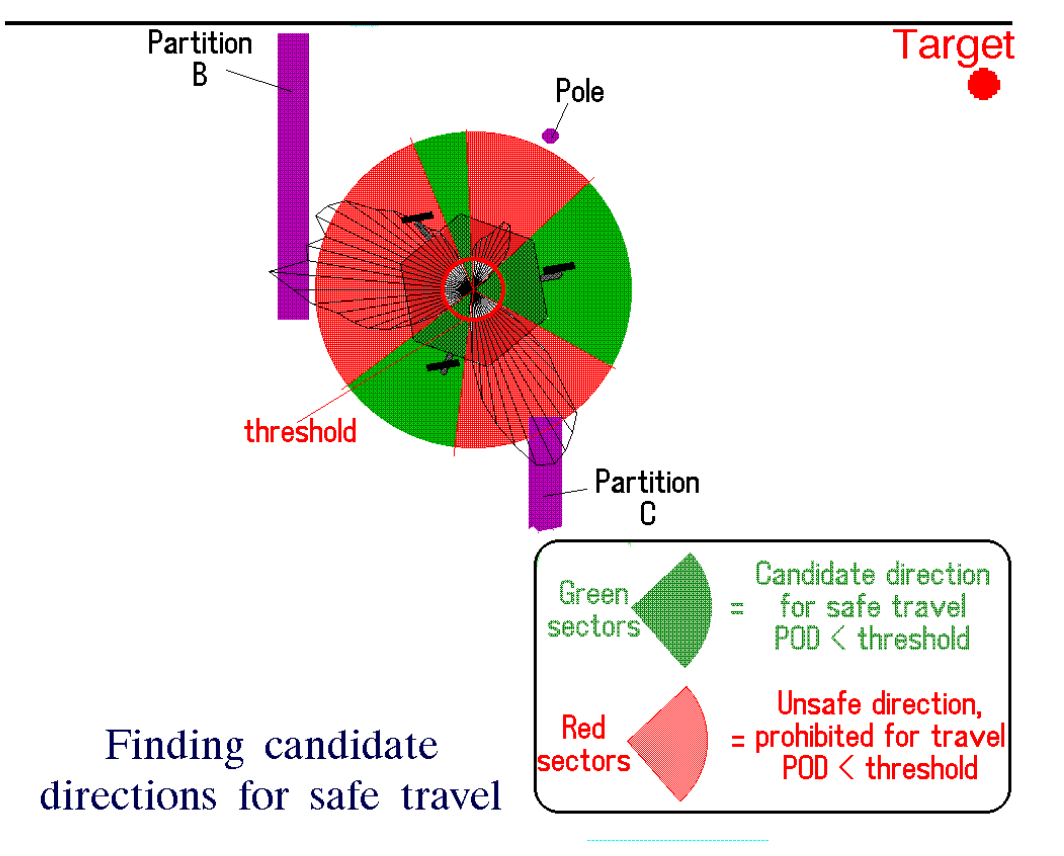
\includegraphics[width=0.6\textwidth]{img/candidate_directions}
    \caption{O limiar de um histograma polar determina as direções candidatas para um viagem segura. Fonte: \cite{c1}}
    \label{fig:cand_direc}
\end{figure}

\subsection{Técnica de Bubble Band}
\label{sec:bubbleband}

A técnica de \textit{Bubble Band} consiste em um método que define uma "bolha", a qual representa a distância livre necessária ao entorno do robô para que ele se desloque sem que haja colisão. A forma da bolha pode variar de acordo com a estrutura do robô, de modo que esta se encaixe na geometria do mesmo.

\begin{figure}[H]
    \centering
    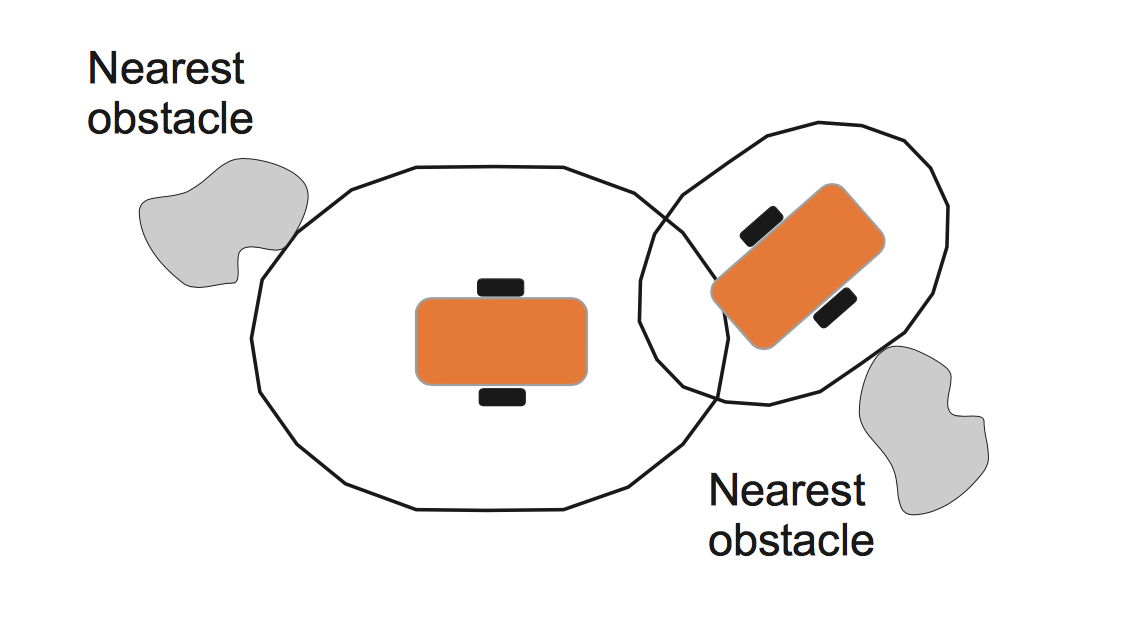
\includegraphics[width=0.6\textwidth]{img/bubble}
    \caption{Técnica de Bubble Band. Fonte: \cite{c2}}
    \label{fig:bubble}
\end{figure}
